\documentclass[12pt,a4paper]{article}
\usepackage[utf8]{inputenc}
\usepackage[T1]{fontenc}
\usepackage[spanish]{babel}
\usepackage{amsmath}
\usepackage{amsfonts}
\usepackage{amssymb}
\usepackage{graphicx}
\usepackage[width=18.00cm, height=26.00cm]{geometry}
\author{Gabriel Octavio Lozano Pinzón}
\title{Laboratorio 10}
\begin{document}
\maketitle
Para este laboratorio usamos la plantilla de Cross-sectional Equity para iterar usando nuestros propios factores. Para tener una linea base, usamos un año y medio desde principios de 2011 a finales de 2012. Esto resulta en los resultados que se muestran en la Figura \ref{fig:lineabase}.\\

Para mejorar el algoritmo vamos a introducir tres variables nuevas, que consisten en el market cap, la opinión de los expertos y un score de mean reversion. Para este ejercicio consideramos que los pesos antes dados no son muy buenos dado su performance, por tanto les bajamos su nivel de importancia con pesos pequeños ademas market cap solo nos filtra el tamaño de la empresa y si bien nos importa no resulta ser un factor determinante cuando se analiza con alpha lens.\\

Cuando se tiene esto en cuenta esto obtenemos el resultado de la Figura 2 en la cual apreciamos un salto en el desempeño del algoritmo. Esto implica que nuestros alpha factors son mejores que la anterior iteración o linea base.  También muestra que el algoritmo no nos hace caer el perdidas, sino que tiende a aprovechar de mejor manera el mercado. \\


\begin{figure}
	\centering
	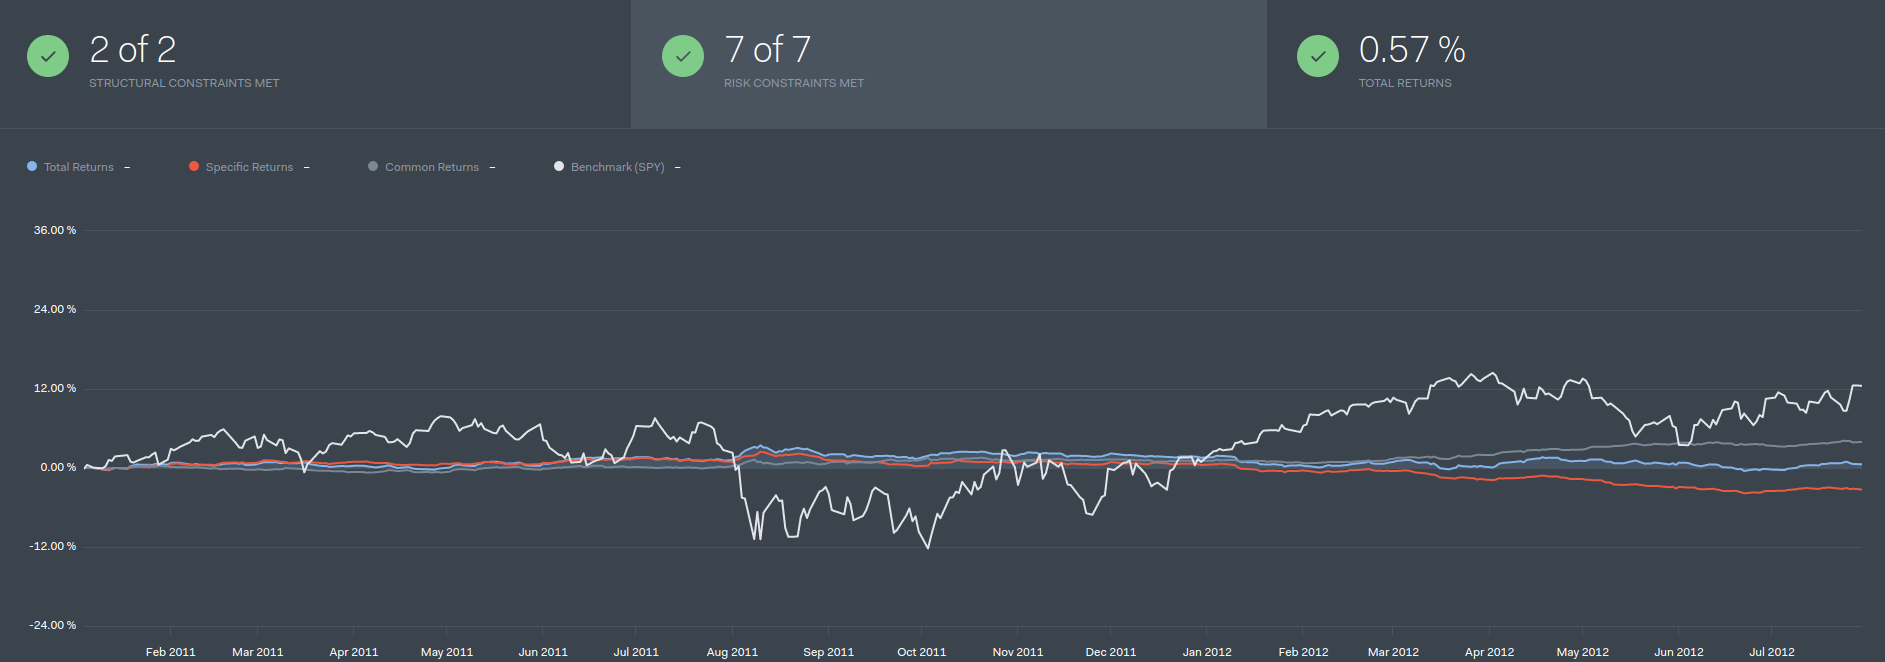
\includegraphics[width=1\linewidth]{linea_base}
	\caption{Resultados de la linea base}
	\label{fig:lineabase}
\end{figure}
\begin{figure}
	\centering
	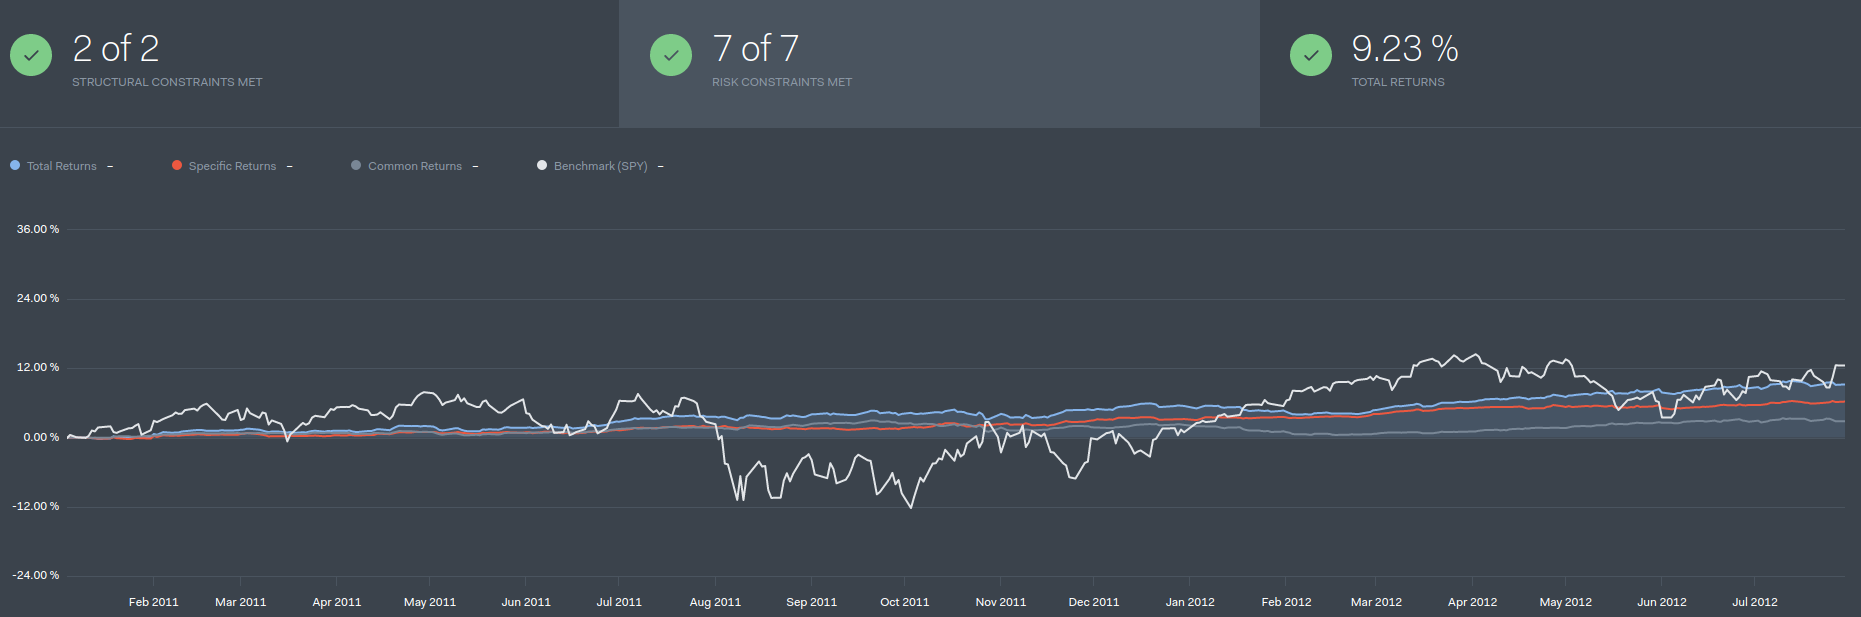
\includegraphics[width=0.7\linewidth]{fase_final}
	\caption{Resultados con los custom Factors y los pesos adecuados}
	\label{fig:fasefinal}
\end{figure}

\end{document}